\section{Availability and Resource Contention\label{sec:4_formulation}}
The charge scheduling framework described in this paper is formulated as a constrained optimization problem that can be solved as a Mixed Integer Linear Program (MILP) of the form
\begin{equation}\label{eqn:MILP}\begin{matrix}
	\underset{\mathbf{y}}{\text{min}} \ \mathbf{y}^T\mathbf{g} \text{ subject to } \\
	\tilde{A}\mathbf{y} = \tilde{\mathbf{b}}, \ A\mathbf{y} \le \mathbf{b},
\end{matrix} \end{equation}
where $\mathbf{y}$, $\tilde{A}$, $A$, and $\mathbf{g}$ represent the solution vector, equality and inequality constraints, and cost vector respectively. In this paper, $\mathbf{y}$ is comprised of several variables, and is expressed as 
\begin{equation}\label{eqn:yDef}
	\mathbf{y} = \begin{bmatrix}
			\boldsymbol{\sigma} \\ 
			\mathbf{c}      \\ 
			\mathbf{s}      \\ 
			\mathbf{h}      \\ 
			\mathbf{k}      \\ 
			\mathbf{r}      \\ 
			\mathbf{g}      \\
			\mathbf{p}      \\ 
			q_{\text{on}}   \\ 
			q_{\text{all}}  \\
		     \end{bmatrix},
\end{equation}
where $\boldsymbol{\sigma}$, $\mathbf{c}$, $\mathbf{s}$, $\mathbf{h}$, $\mathbf{k}$, $\mathbf{r}$, $\mathbf{p}$, $q_{\text{on}}$, and $q_{\text{all}}$ will be developed through the course of this paper.
\par The cost function in \eqref{eqn:MILP} will be designed to model a realistic billing structure used by \cite{rocky_mountain_power_rocky_2021} and minimises the cost even in the presence of uncontrolled loads. Additionally, the constraints are designed to encorporate bus schedules, limit bus state of charges, and include a linear charge model calibrated on data from the Utah Transit Authority.
\subsection{Setup}
\par A solution to the bus charge problem includes both temporal and categorical information. The temporal aspect shows when and for how long a bus should charge and the categorical shows which bus must charge, indicating a solution with two dimensions.  The first dimension represents time continuously from left to right, and the second describes the buses as shown in Fig. \ref{fig:busTime1}.
\begin{figure*}
	\centering
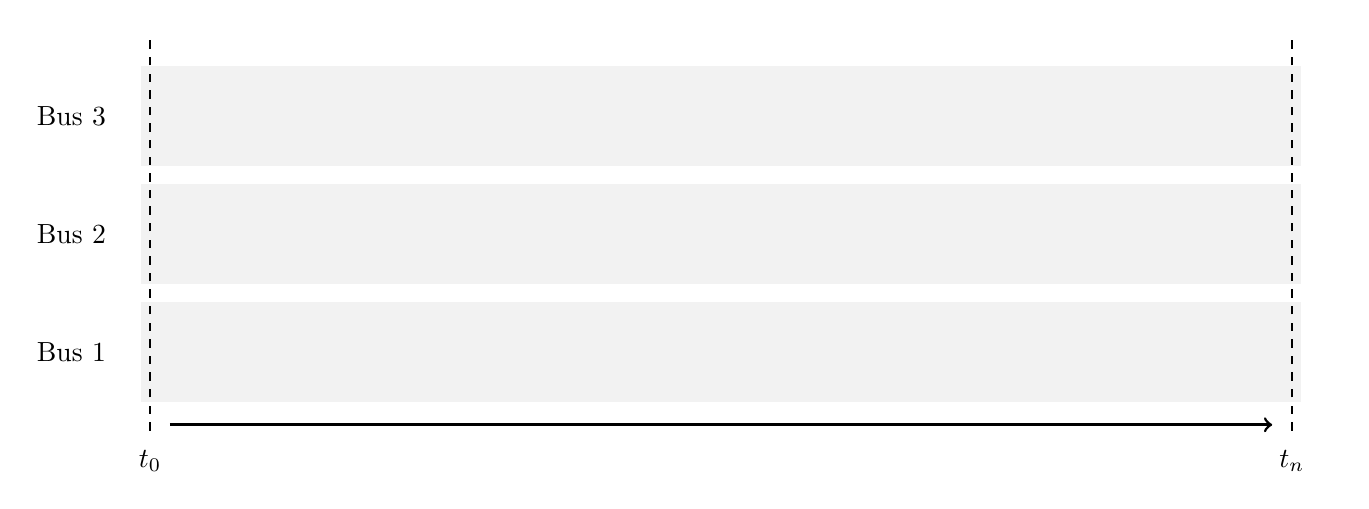
\begin{tikzpicture}
	\node[rectangle, fill=gray!10, minimum width=5.8in, minimum height=0.5in](bus1Box) at (7.75,1){};
	\node(bus1BoxLabel) at (-0.5, 1){Bus 1}; 

	\node[rectangle, fill=gray!10, minimum width=5.8in, minimum height=0.5in](bus2Box) at (7.75,2.5){};
	\node(bus1BoxLabel) at (-0.5, 2.5){Bus 2};

	\node[rectangle, fill=gray!10, minimum width=5.8in, minimum height=0.5in](bus3Box) at (7.75,4){};
	\node(bus1BoxLabel) at (-0.5, 4){Bus 3};

	\node[label=below:$t_0$](origin) at (0.5,0){};
	\node(yAxes) at (15.5,0){};
	\node(xAxes) at (0.5,5){};
	\node[label=below:$t_n$](bottomRight) at (15,0){};
	\node(topRight) at (15,5){};
	\draw[dashed, line width=0.5pt] (origin.center) -- (xAxes.center); 
	\draw[dashed, line width=0.5pt] (bottomRight.center) -- (topRight.center);
	\node(t0) at (0.75,-0.05){};
	\node(tn) at (14.75,-0.05){};
	\draw[->, line width=1pt] (t0.north) -- (tn.north); 
\end{tikzpicture}
	\caption{Description of the bus and time axis}
	\label{fig:busTime1}
\end{figure*}

\par Each bus follows a schedule of arrival and departure times, where the $i^{\text{th}}$ bus's $j^{\text{th}}$ stop begins at arrival time $a_{ij}$ and terminates at departure time $d_{ij}$ (see Fig. \ref{fig:busTime3}).  A bus can be assigned to charge anytime the bus is in the station such that the charge start time, $c_{ij}$, is greater than or equal to $a_{ij}$, and the charge stop time, $s_{ij}$, is less than the departure time $d_{ij}$ as shown in Fig. \ref{fig:busTime3}. In the context of a MILP, the arrival and departure times $a_{ij}$ and $d_{ij}$ are known ahead of time and charge times $c_{ij}$ and $s_{ij}$ are optimization variables. 
\begin{figure*}
\centering
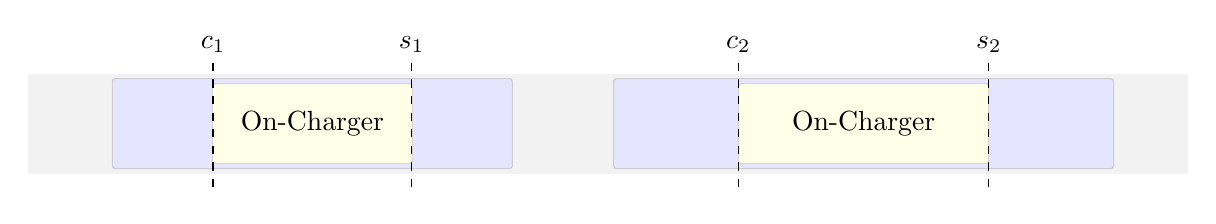
\begin{tikzpicture} 
	\node[rectangle, fill=gray!10, minimum width=5.8in, minimum height=0.5in](busSched) at (7.75,1){}; 

	\node[rectangle, draw=blue!10!black!20, fill=blue!10, minimum width=2in, minimum height=0.45in, rounded corners=1pt](busAvail1) at (4,1){In-Station};
	\node[rectangle, draw=blue!10!black!20, fill=blue!10, minimum width=2.5in, minimum height=0.45in, rounded corners=1pt](busAvail2) at (11,1){In-Station};

	\node[rectangle, draw=yellow!10!black!20, fill=yellow!10, minimum width=1in, minimum height=0.4in, rounded corners=1pt](busAvail1) at (4,1){On-Charger};
	\node[rectangle, draw=yellow!10!black!20, fill=yellow!10, minimum width=1.25in, minimum height=0.4in, rounded corners=1pt](busAvail2) at (11,1){On-Charger};


	\node(firstATop) at (2.74,2){$c_1$};
	\node(firstABtm) at (2.74,0.2){};
	\draw[dashed, line width=0.5pt](firstATop) -- (firstABtm.center);
	\node(firstDTop) at (5.26,2){$s_1$};
	\node(firstDBtm) at (5.26,0.2){};
	\draw[dashed, line width=0.5pt](firstDTop) -- (firstDBtm.center);

	\node(secondATop) at (9.41,2){$c_2$};
	\node(secondABtm) at (9.41,0.2){};
	\draw[dashed, line width=0.5pt](secondATop) -- (secondABtm.center);
	\node(secondDTop) at (12.59,2){$s_2$};
	\node(secondDBtm) at (12.59,0.2){};
	\draw[dashed, line width=0.5pt](secondDTop) -- (secondDBtm.center);


\end{tikzpicture}
\caption{Bus Charging}
\label{fig:busTime3}
\end{figure*}

\subsection{Constraints}
The relationship between the arrival, departure, and charge intervals for the $i^{\text{th}}$ bus at the $j^{\text{th}}$ stop can be expressed as a set of inequality constraints such that
\begin{equation}\begin{aligned}
	a_{ij} &< c_{ij} \\
	c_{ij} &< s_{ij} \\
	s_{ij} &< d_{ij}.
\end{aligned}\end{equation}
These constraints can be rewritten such that the optimization variables are on the left, the known parameters are on the right, and the relationship is "less than" (or standard form) such that
\begin{equation}\begin{aligned}
	-c_{ij} &< -a_{ij}\\
	c_{ij} - s_{ij} &< 0\\
	s_{ij} &< d_{ij}.
\end{aligned}\end{equation}
Standard form is preferred because it provides a standard way to represent equations. Having the optimization variables on the left also allows the expression to be written using matrix notation as 
\begin{equation}\label{eqn:timeConstraint}
	\begin{bmatrix} -1 & 0 \\
	                 1 & -1 \\
		0 & 1\end{bmatrix} \begin{bmatrix} c_{ij} \\ s_{ij}\end{bmatrix} \le \begin{bmatrix}-a_{ij} \\ 0 \\ d_{ij} \end{bmatrix}.
\end{equation}
	However, because all constraints must follow the form $A\mathbf{y} = \mathbf{b}$ as shown in \eqref{eqn:MILP}, \eqref{eqn:timeConstraint} is expressed in terms of $\mathbf{y}$ such that
\begin{equation} \begin{aligned}
	\begin{bmatrix}
		-1^c_{ij} & 0 & \hdots &  0        \\
	         1^c_{ij} & 0 & \hdots & -1^d_{ij} \\
		 0        & 0 & \hdots &  1^d_{ij} \\ 
	\end{bmatrix}
	\mathbf{y} &\le 
	\begin{bmatrix}
	        -a_{ij} \\ 
		 0      \\ 
		 d_{ij} \\
	\end{bmatrix} \ \forall i,j \\
	A_1\mathbf{y} &\le \mathbf{b}_1,
\end{aligned} \end{equation}
	where $1^c_{ij}$ is $1$ at the location corresponding to $c_{ij}$, $1^d_{ij}$ is $1$ at the location corresponding to $d_{ij}$, and $A_1$ and $\mathbf{b}_1$ stack the constraints given in \eqref{eqn:timeConstraint} for all $i,j$.
	\par The decision variables $s_{ij}$ and $c_{ij}$ from \eqref{eqn:timeConstraint} show when a bus must start and finish charging, but do not indicate on which charger. The variable $\boldsymbol{\sigma}$ from \eqref{eqn:yDef} is a vector of binary variables. Each element of $\boldsymbol{\sigma}$ is denoted $\sigma_{ijk}$ and is $1$ when bus $i$ charges during the $j^{\text{th}}$ stop at charger $k$. Because a bus can only charge at one charger at a time, the values in $\boldsymbol{\sigma}$ must be constrained such that
\begin{equation}
	\begin{aligned}
		\sum_k \sigma_{ijk} \le 1 \ \forall i,j
	\end{aligned}
\end{equation} 
or in standard form as 
\begin{equation} \begin{aligned}
	\begin{bmatrix}1_{ij1} & 0 & \hdots & 0 & 1_{ijk} \end{bmatrix} \mathbf{y} &\le \mathbf{1} \ \forall i,j\\
		A_2\mathbf{y} & \le \mathbf{b}_2,
\end{aligned} \end{equation}
where $1_{ijk}$ represents a $1$ at the location corresponding to $\sigma_{ijk}$.
	The variable $\sigma_{ijk}$ is used in several scenarios. The first is to ensure that buses without charge assignments have a charge time of zero by constraining $s_{ij}$ and $c_{ij}$ to be the same value. This is done by letting
	\begin{equation}\label{eqn:A3}\begin{aligned}
	s_{ij} - c_{ij} &\le M\sum_{k}\sigma_{ijk} \\
	s_{ij} - c_{ij} - \sum_{k}\sigma_{ijk}M &\le 0\\
	\begin{bmatrix} 1_s & -1_c & -M_{\sigma} \end{bmatrix}\begin{bmatrix}s_{ij} \\ c_{ij} \\ \sigma_{ij1} \\ \vdots \\ \sigma_{ijk} \end{bmatrix} &\le 0 \ \forall i,j 
\end{aligned} \end{equation}
	where $M$ is the maximum difference between $s_{ij}$ and $c_{ij}$, or the number of seconds in a day, denoted $\text{nTime}$ and $M_\sigma$ represents multiple values of $M$ at locations corresponding to each $\sigma_{ijk}$. The constraints in \refeq{eqn:A3} can be appropriately zero padded and stacked for all $i,j$ to form the linear expression
	\begin{equation} 
		A_3\mathbf{y} \le \mathbf{b}_3
	\end{equation}
	\par The values in $\boldsymbol{\sigma}$, $\mathbf{c}$, and $\mathbf{s}$ form a complete charge plan representation were $c_{ij}$ and $s_{ij}$ describe time periods when a bus will charge and $\sigma_{ijk}$ gives which charger to use. (see Fig. \ref{fig:busTime4}).
\begin{figure*}
	\centering
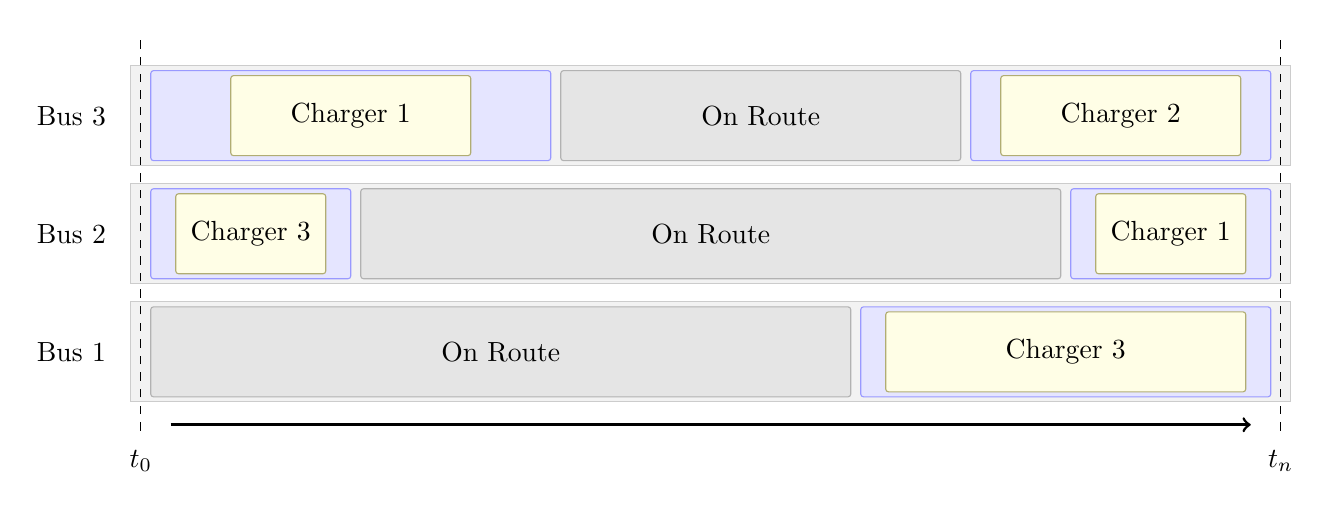
\begin{tikzpicture}
	\node[rectangle, draw=gray!40, fill=gray!10, minimum width=5.8in, minimum height=0.5in](charger1Box) at (3in,1){};
	\node(bus1BoxLabel) at (-0.5, 1){Bus 1}; 

	\node[rectangle, draw=gray!40, fill=gray!10, minimum width=5.8in, minimum height=0.5in](charger2Box) at (3in,2.5){};
	\node(bus1BoxLabel) at (-0.5, 2.5){Bus 2};

	\node[rectangle, draw=gray!40, fill=gray!10, minimum width=5.8in, minimum height=0.5in](charger3Box) at (3in,4){};
	\node(bus1BoxLabel) at (-0.5, 4){Bus 3};

	\node[label=below:$t_0$](origin) at (0.15in,0){};
	\node(xAxes) at (0.15in,5){};
	\node[label=below:$t_n$](bottomRight) at (5.85in,0){};
	\node(topRight) at (5.85in,5){};
	\draw[dashed, line width=0.5pt] (origin.center) -- (xAxes.center); 
	\draw[dashed, line width=0.5pt] (bottomRight.center) -- (topRight.center);
	\node(t0) at (0.3in,-0.05){};
	\node(tn) at (5.7in,-0.05){};
	\draw[->, line width=1pt] (t0.north) -- (tn.north); 

	% draw bus 3 boxes
	\node[rectangle, draw=blue!40, fill=blue!10, minimum width=2in, minimum height=0.45in, rounded corners=1pt](bus1Avail1) at (1.2in,4){};
	\node[rectangle, draw=yellow!50!black!70, fill=yellow!10, minimum width=1.2in, minimum height=0.4in, rounded corners=1pt](bus1Time1) at (1.2in,4){Charger 1};

	\node[rectangle, draw=black!30, fill=black!10, minimum width=2in, minimum height=0.45in, rounded corners=1pt](bus2Time1) at (3.25in,4){On Route};

	\node[rectangle, draw=blue!40, fill=blue!10, minimum width=1.5in, minimum height=0.45in, rounded corners=1pt](bus1Avail1) at (5.05in,4){};
	\node[rectangle, draw=yellow!50!black!70, fill=yellow!10, minimum width=1.2in, minimum height=0.40in, rounded corners=1pt](bus3Time1) at (5.05in,4){Charger 2};

	% draw bus 2 boxes
	\node[rectangle, draw=blue!40, fill=blue!10, minimum width=1in, minimum height=0.45in, rounded corners=1pt](bus1Avail1) at (0.7in,2.5){};
	\node[rectangle, draw=yellow!50!black!70, fill=yellow!10, minimum width=0.75in, minimum height=0.4in, rounded corners=1pt](free1) at (0.7in,2.5){Charger 3};

	\node[rectangle, draw=black!30, fill=black!10, minimum width=3.5in, minimum height=0.45in, rounded corners=1pt](bus3Time2) at (3.0in,2.5){On Route};

	\node[rectangle, draw=blue!40, fill=blue!10, minimum width=1.0in, minimum height=0.45in, rounded corners=1pt](bus1Avail1) at (5.3in,2.5){};
	\node[rectangle, draw=yellow!50!black!70, fill=yellow!10, minimum width=0.75in, minimum height=0.4in, rounded corners=1pt](free2) at (5.3in,2.5){Charger 1};

	% draw bus 1 boxes 
	\node[rectangle, draw=black!30!, fill=black!10, minimum width=3.5in, minimum height=0.45in, rounded corners=1pt](bus3Time2) at (1.95in,1){On Route}; 

	\node[rectangle, draw=blue!40, fill=blue!10, minimum width=2.05in, minimum height=0.45in, rounded corners=1pt](bus1Avail1) at (4.775in,1){};
	\node[rectangle, draw=yellow!50!black!70, fill=yellow!10, minimum width=1.8in, minimum height=0.4in, rounded corners=1pt](bus1Time2) at (4.775in,1){Charger 3};
\end{tikzpicture}
	\caption{Reserving time slots on chargers}
	\label{fig:busTime4}
\end{figure*}

The variable $\sigma_{ijk}$ is also necessary to eliminate situations where more then one bus is assigned to a charger at the same time. Note that this can only happen when $a_{ij}$ for bus $i$ is less than $d_{i^{'}j^{'}}$ for bus $i^{'}$ as shown in Fig. \ref{fig:potentialOverlap}. Charging overlap can be avoided by constraining
\begin{figure}
	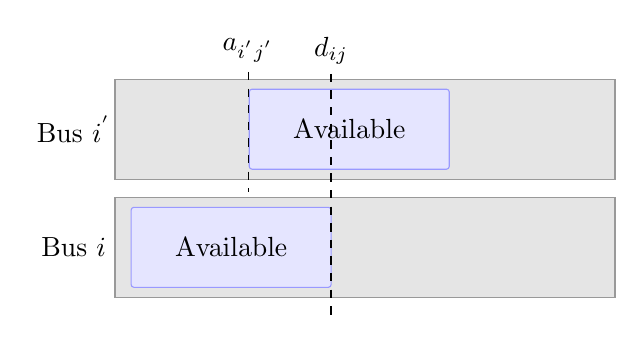
\begin{tikzpicture} 
		\node[rectangle, draw=black!40, fill=black!10, minimum width=2.5in, minimum height=0.5in](charger1Box) at (3.2,1){};
		\node(bus1BoxLabel) at (-0.5, 1){Bus $i$}; 
		\node[rectangle, draw=black!40, fill=black!10, minimum width=2.5in, minimum height=0.5in](charger2Box) at (3.2,2.5){};
		\node(bus1BoxLabel) at (-0.5, 2.5){Bus $i^{'}$};
		\node[rectangle, draw=blue!40, fill=blue!10, minimum width=1in, minimum height=0.4in, rounded corners=1pt] at (1.5,1){Available};
		\node[rectangle, draw=blue!40, fill=blue!10, minimum width=1in, minimum height=0.4in, rounded corners=1pt] at (3,2.5){Available};
		\node(aJPrimeHigh) at (1.72,3.5){$a_{i^{'}j^{'}}$};
		\node(aJPrimeLow) at (1.72,1.7){};
		\node(dJHigh) at (2.77,3.5){$d_{ij}$};
		\node(dJLow) at (2.77,0.0){};
		\draw[dashed, line width=0.5pt] (aJPrimeHigh) -- (aJPrimeLow.center);
		\draw[dashed, line width=0.5pt] (dJHigh) -- (dJLow);
	\end{tikzpicture}
	\caption{Potential Overlap}
	\label{fig:potentialOverlap}
\end{figure}



\begin{equation}\label{eqn:overlapConstraints1}
	\begin{array}{c}
		c_{i^{`}j^{`}} > s_{ij} \\
		\text{or} \\
		c_{ij} > s_{i^{`}j^{`}} 
	\end{array} \ \forall ij
\end{equation}
	Let $l_{iji^{`}j^{`}}$ be a binary decision variable that is $1$ when $c_{i^{'}j^{'}} > s_{ij}$, and $0$ when $c_{ij} > s_{i^{'}j^{'}}$. The expression from \refeq{eqn:overlapConstraints1} can be rewritten as
\begin{equation} \begin{aligned}
	c_{i^{`}j^{`}} - s_{ij}  &> -Ml_{iji^{`}j^{`}}\\
	c_{ij}-s_{i^{`}j^{`}} &>  -M(1 - l_{iji^{`}j^{`}})
\end{aligned}\end{equation}
	However, this constraint is only necessary when buses $i$ and $i^{`}$ must use the same charger. This can be remedied as
\begin{equation}\label{eqn:overlapConstraints2}\begin{aligned}
	c_{i^{'}j^{'}} - s_{ij} &> M\left[(\sigma_{i^{'}j^{'}k} + \sigma_{ijk}) - 2\right] - Ml_{iji^{`}j^{`}} \ \forall k \\
	c_{ij} - s_{i^{'}j^{'}} &> M\left[(\sigma_{i^{'}j^{'}k} + \sigma_{ijk}) - 2\right] - M(1 - l_{iji^{`}j^{`}})\ \forall k \\
\end{aligned}\end{equation}
When $(\sigma_{i^{'}j^{'}k} + \sigma_{ijk}) < 2$, \eqref{eqn:overlapConstraints2} is trivially satisfied for all values of $c_{i^{'}j^{'}}$ and $s_{ij}$. When $\sigma_{i^{'}j^{'}k} = \sigma_{ijk} = 1$, \eqref{eqn:overlapConstraints2} simplifies to \eqref{eqn:overlapConstraints1}. Equation \eqref{eqn:overlapConstraints2} can be expressed in standard form as 
	\begin{equation}\label{eqn:overlapConstraints3}\begin{aligned}
		-c_{i^{`}j^{`}} + s_{ij} + M\sigma_{i^{'}j^{'}k} + M\sigma_{ijk} - Ml_{iji^{`}j^{`}}&\le 2M  \ \forall k\\
		-c_{ij} + s_{i^{`}j^{`}} + M\sigma_{i^{'}j^{'}k} + M\sigma_{ijk} + Ml_{iji^{`}j^{`}}&\le 3M  \ \forall k\\
	\end{aligned}\end{equation}
	and finally as
	\begin{equation}\begin{aligned} 
		\begin{bmatrix} 
			-1 & 0 &  0 & 1 & M & M & -M \\
			 0 & 1 & -1 & 0 & M & M &  M \\
		\end{bmatrix} 
		\begin{bmatrix}
			c_{i^{'}j^{'}}       \\ 
			s_{i^{'}j^{'}}       \\
			c_{ij}               \\
			s_{ij}               \\ 
			\sigma_{i^{'}j^{'}k} \\ 
			\sigma_{ijk}         \\
			l_{iji^{`}j^{`}}     \\
		\end{bmatrix} &\le 
		\begin{bmatrix} 
			2M \\ 
			3M \\
		\end{bmatrix} \forall k
	\end{aligned} \end{equation}
	The constraints in \eqref{eqn:overlapConstraints3} can be repeated for all instances where overlap is possible and concatenated into a single matrix such that
	\begin{equation}\begin{aligned} 
		A_4\mathbf{y} & \le \mathbf{b}_4 \\
	\end{aligned} \end{equation} 
